\documentclass[]{ctexart}

\usepackage{fontspec}
\usepackage{geometry}
\usepackage{setspace}
\usepackage{fancyhdr}
\usepackage{graphicx}
\usepackage{subcaption}
\usepackage{xcolor}

\usepackage{float}       % 支持 [H] 参数强制表格位置
\usepackage{caption}     % 设置表格标题样式
\usepackage{booktabs}    % (可选)增强表格线条美观
\usepackage{longtable}   % (可选)支持跨页表格
\usepackage{amsmath}     % (可选)支持数学表达式
\usepackage{amssymb}     % (可选)增强数学符号
\usepackage{listings}    % (可选)若后续插入IR代码块
\usepackage{hyperref}
\usepackage{array}
\usepackage{tabularx}
\usepackage{longtable}

\author{胡临天}
\date{\today}
\title{论文写作指导作业1}


\begin{document}
\maketitle

% TODO 根据5个关键字检索论文
%       1. 多模态计算
%       2. 可重构计算
%       3. 神经网络量化及剪枝
%       4. 范在网络 
%       5. 边缘计算
% 
%   要求:
%       1. 检索流程:截图+文字
%       2. 作者信息、收录情况、影响因子、被引情况

\section{英文论文检索}
搜索IEEE Xpolre并进入IEEE Xpolor,其界面如图\ref{fig_ieee_xpolor}所示,中选ADVANCED SEARCH然后在Search term中输入关键词,其界面如图\ref{adv_search}。找到需要的论文点进去进入到论文的界面后点红色的PDF下载论文,其界面如图\ref{the_papre}所示。

    \begin{figure}[H]
        \centering
        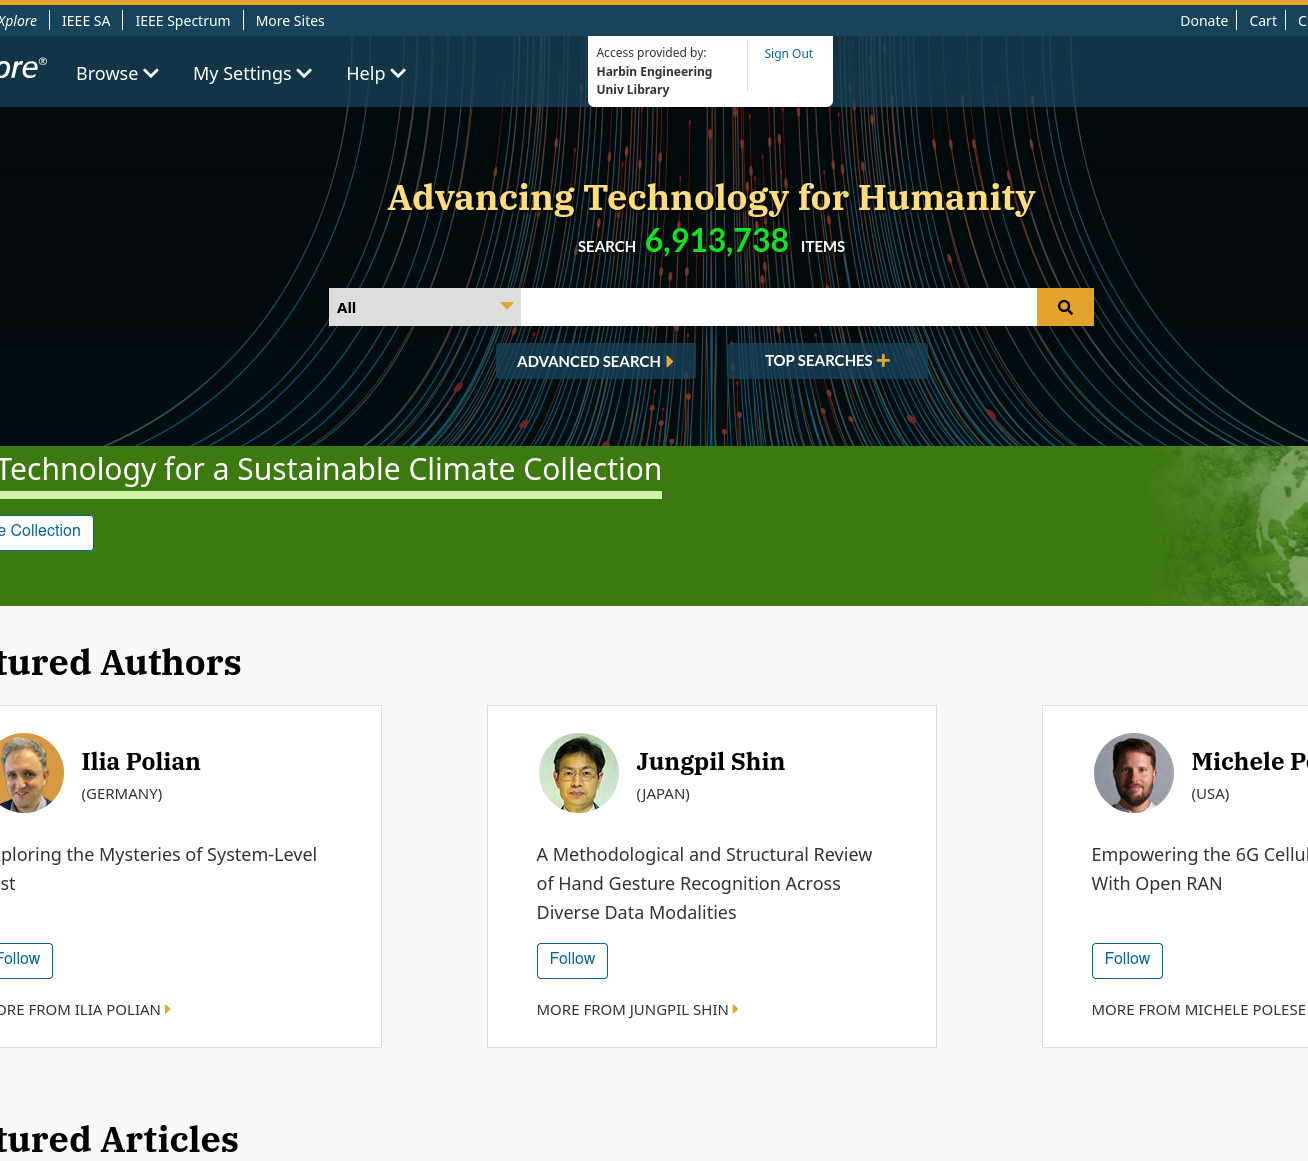
\includegraphics[width=0.5\textwidth]{./asserts/ieee_xpolre.png}
        \caption{IEEE Xpolre界面}
        \label{fig_ieee_xpolor}
    \end{figure}

    % \hfill

    \begin{figure}[H]
        \centering
        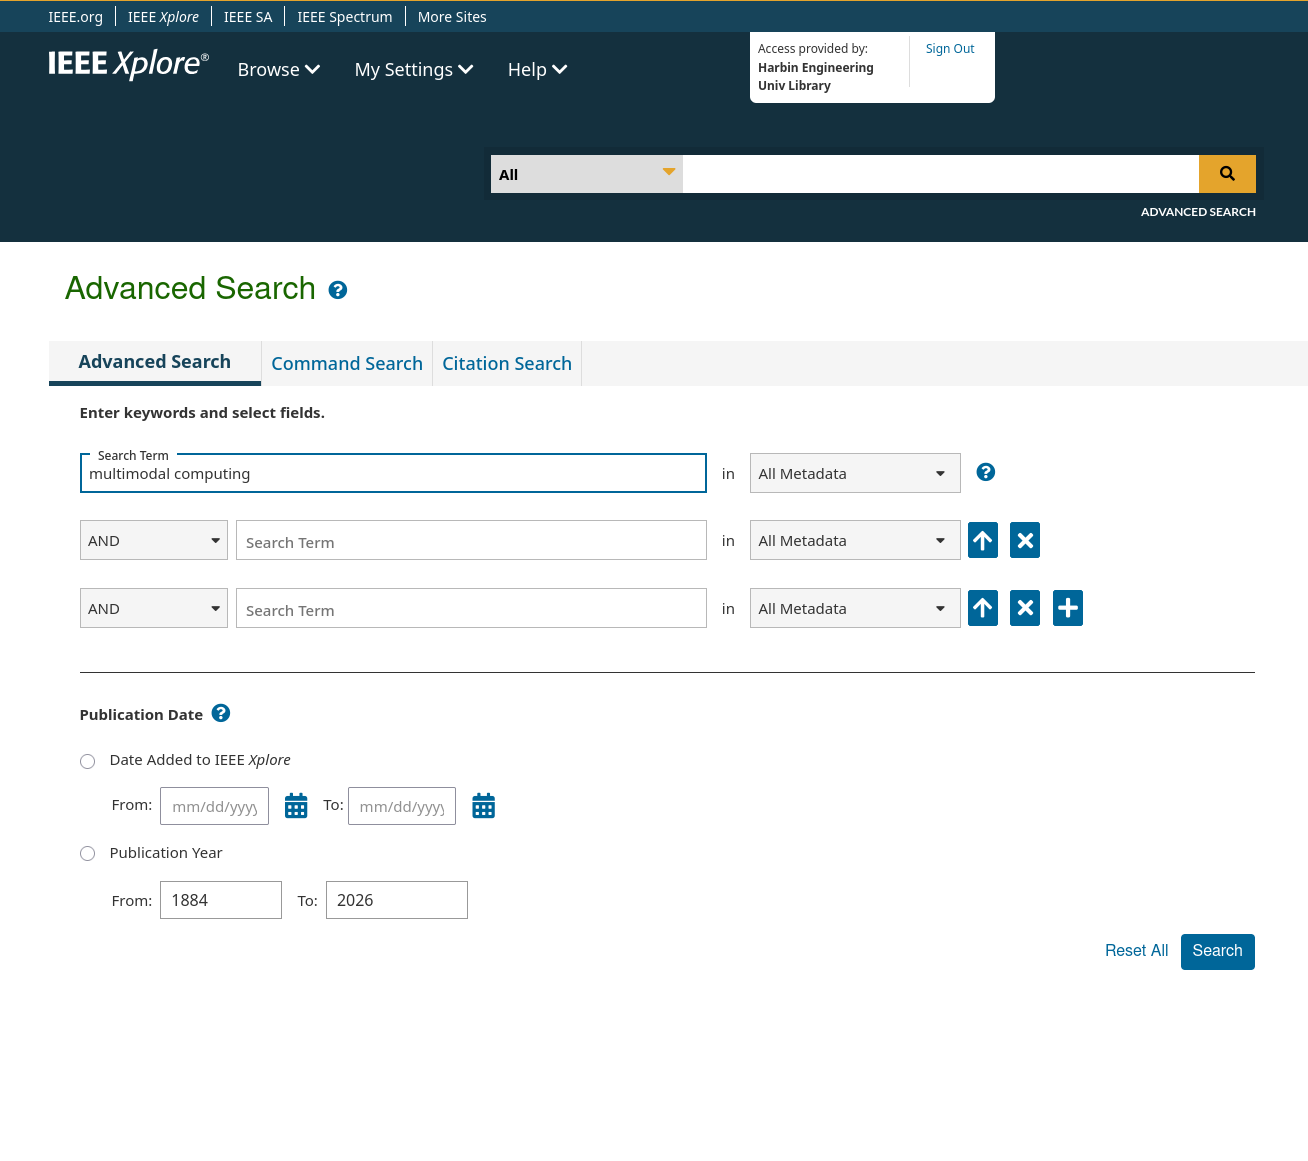
\includegraphics[width=0.5\textwidth]{./asserts/en_search_multi_modal.png}
        \caption{Advanced search界面}
        \label{adv_search}
    \end{figure}

    \begin{figure}[H]
        \centering
        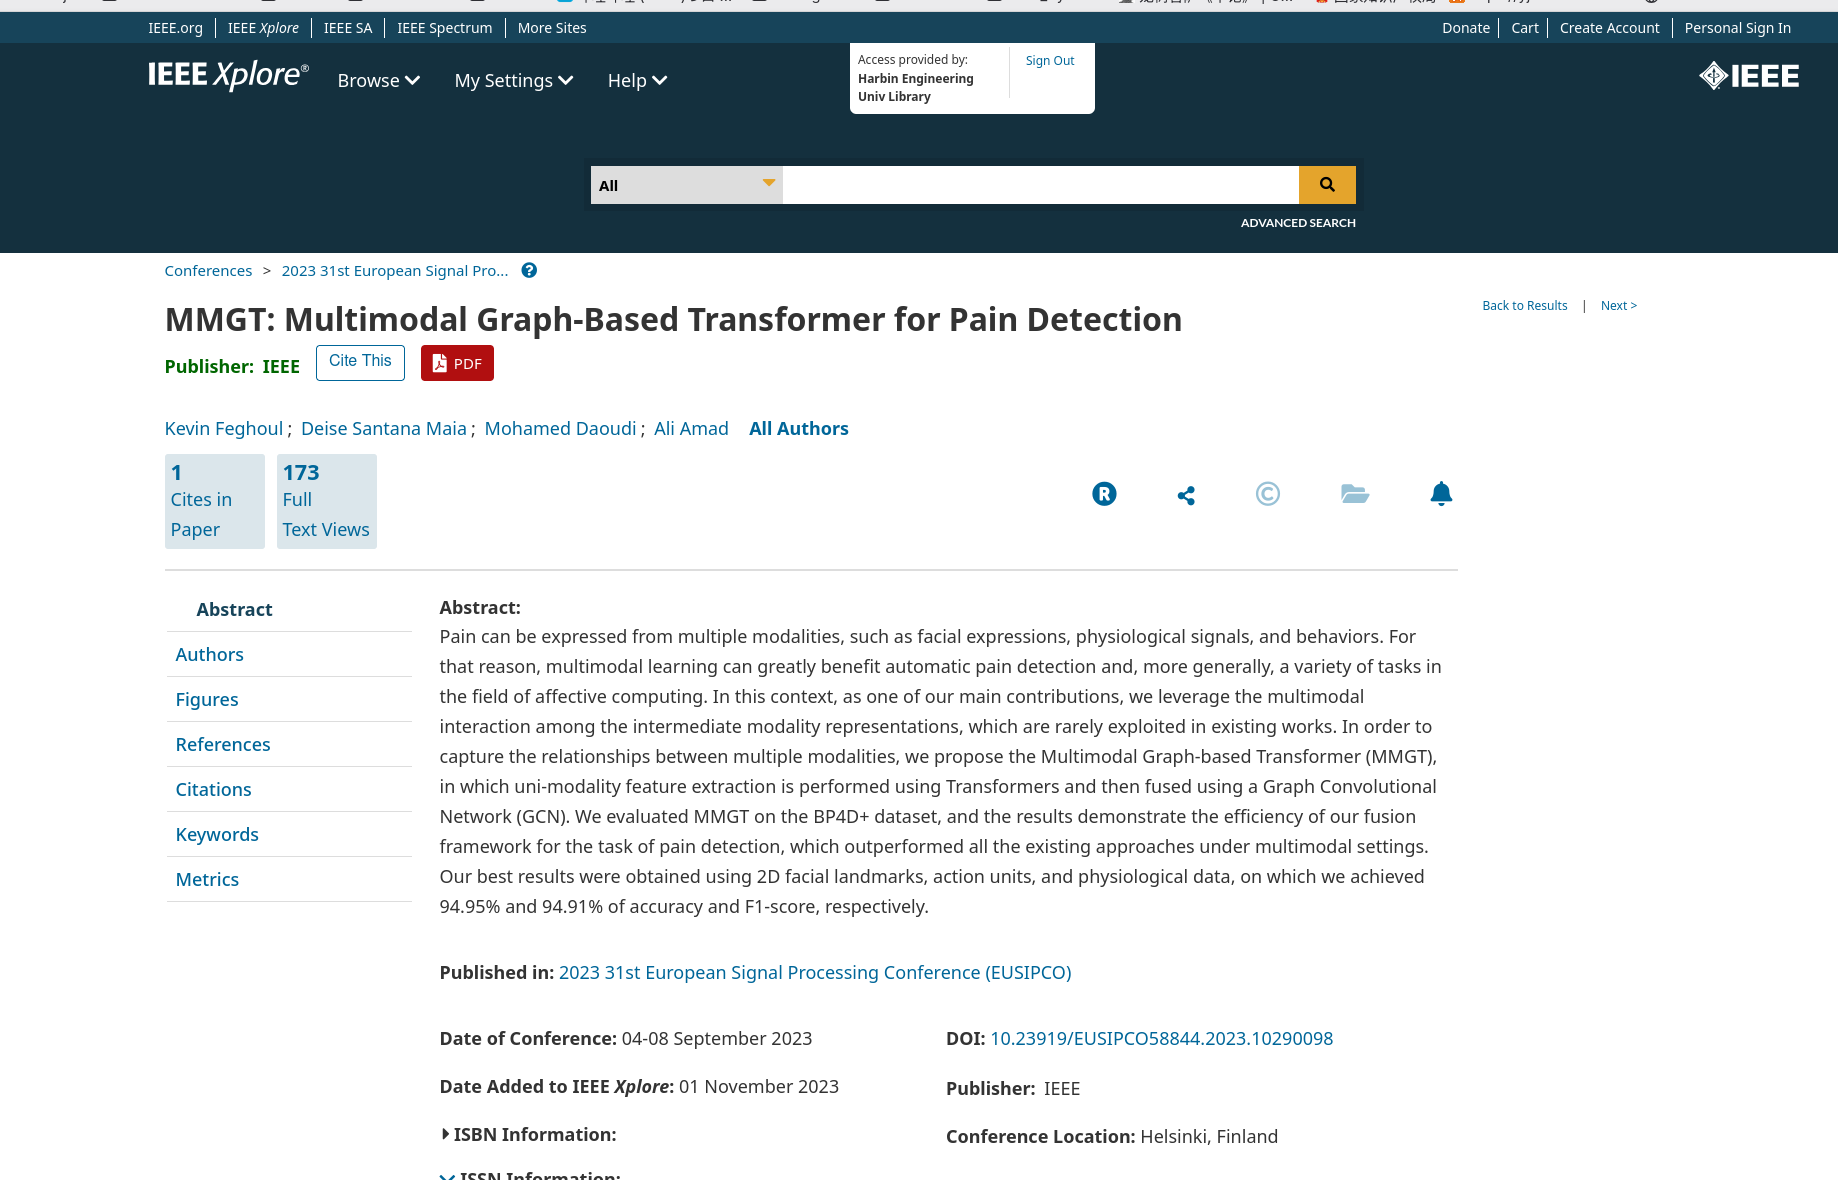
\includegraphics[width=0.5\textwidth]{./asserts/find_the_paper.png}
        \caption{具体的论文界面}
        \label{the_papre}
    \end{figure}







\section{可重构计算}

\subsection{英文论文}

搜索关键词问可重构计算的英文论文的过程为,在IEEE xplore的ADVANCED SEARCH中输入reconfigurable computing,然后点击搜索。

\begin{figure}[H]
    \centering
    \begin{subfigure}{0.8\textwidth}
        \centering
        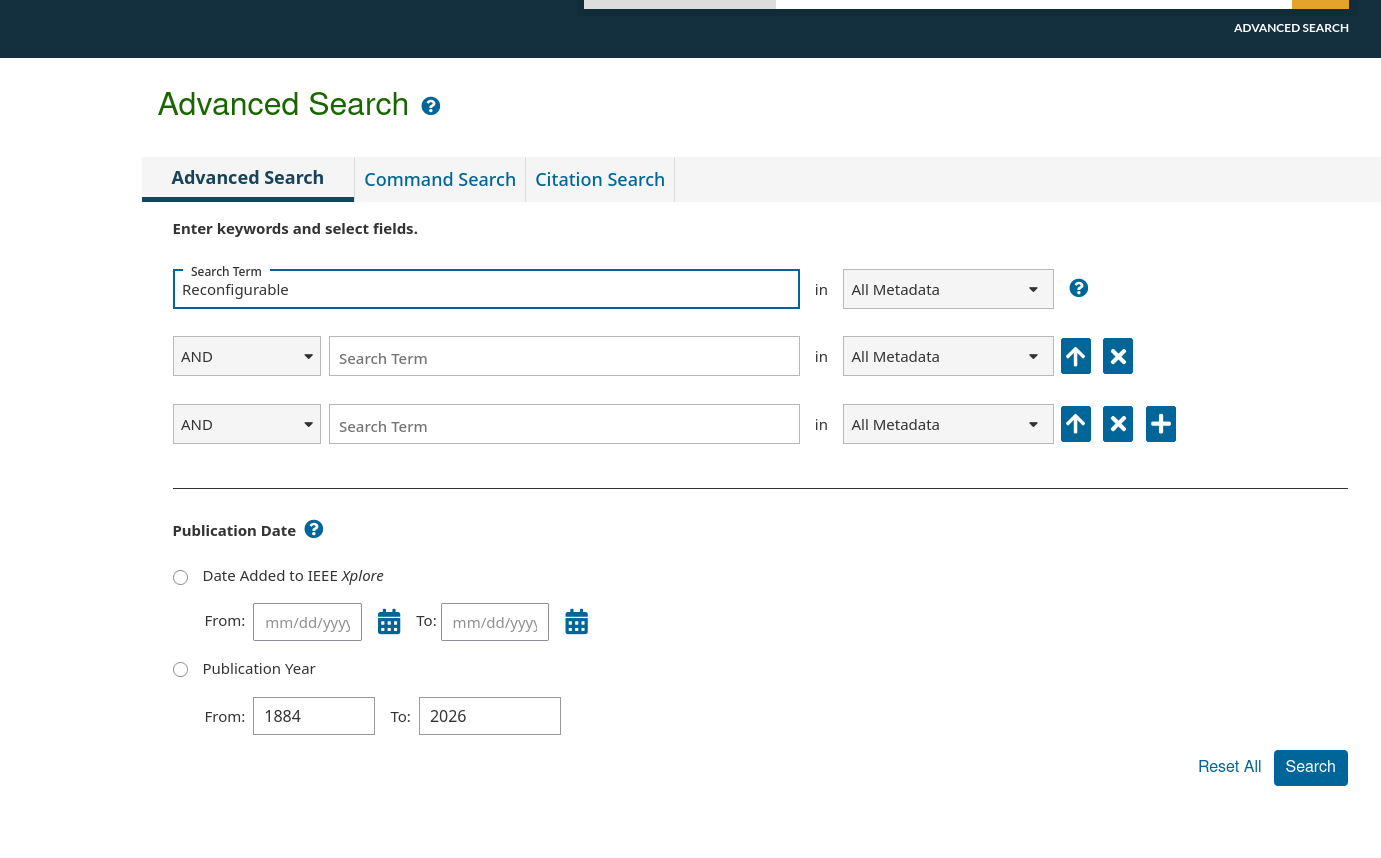
\includegraphics[width=0.7\textwidth]{./asserts/reconfigurable_computing_search.png}
        \caption{Advanced search}
    \end{subfigure}

    % \hfill

    \begin{subfigure}{0.8\textwidth}
        \centering
        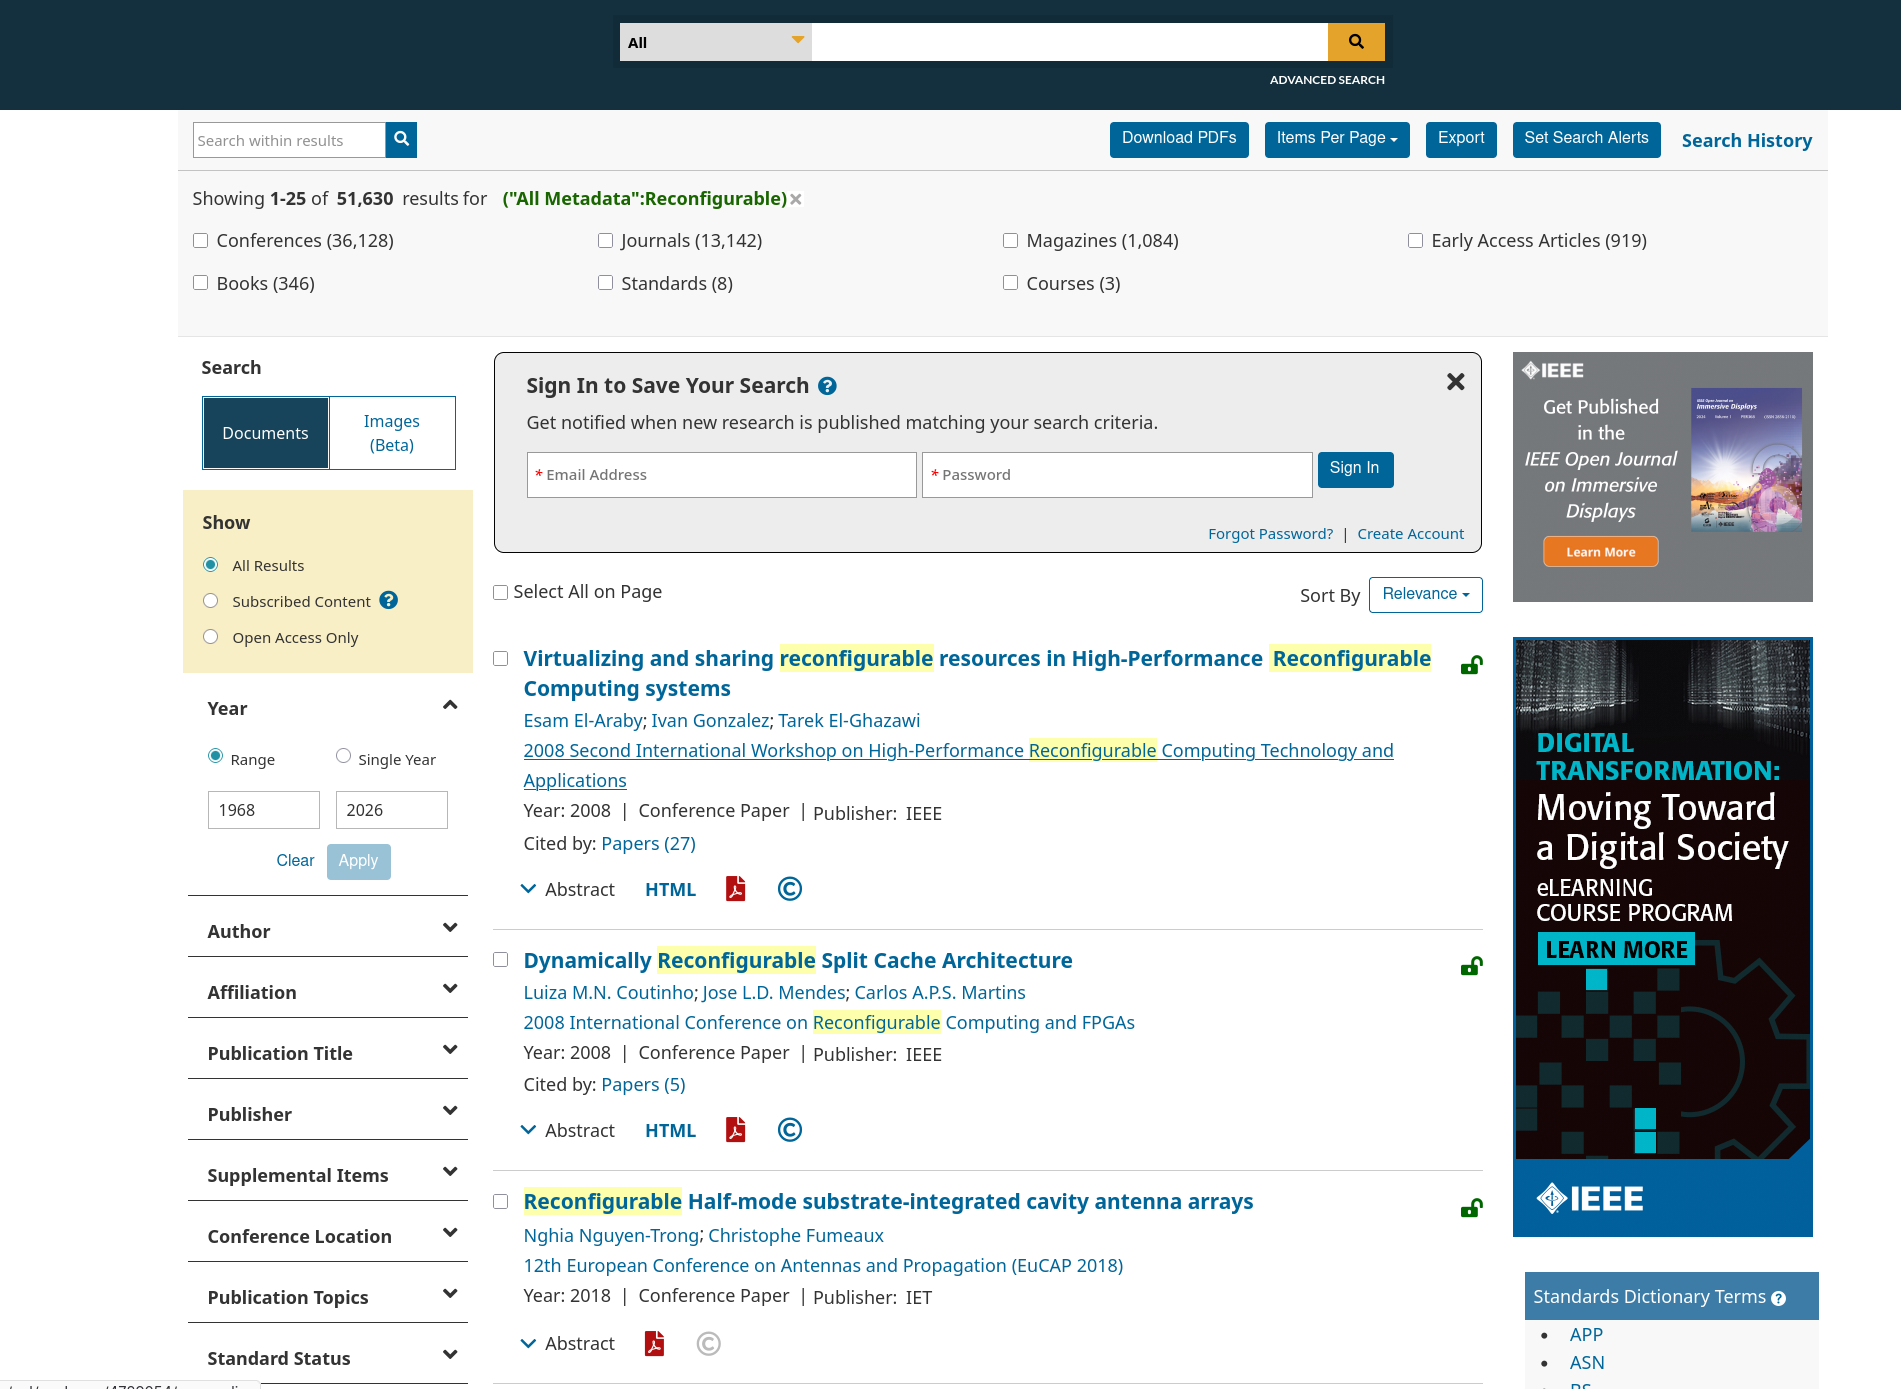
\includegraphics[width=0.7\textwidth]{./asserts/reconfg_res_en.png}
        \caption{Search result}
    \end{subfigure}
\end{figure}


\begin{itemize}
    % 论文题目
    \item 论文名:Resource Awareness FPGA Design Practices for Reconfigurable Computing: Principles and Examples

    % 作者信息
    \item 作者信息:
        \begin{enumerate}
            \item Jinyuan Wu:
                \begin{itemize}
                    \item Fenni National Accelerator Laboratory, Batavia, IL, USA
                \end{itemize}
        \end{enumerate}

    % 收录信息(会议 / 期刊)
    \item 收录情况:
        \begin{itemize}
            \item Published in: 2007 15th IEEE-NPSS Real-Time Conference
            \item DOI: 10.1109/RTC.2007.4382752
        \end{itemize}

    % 影响因子(若是会议则标明“无影响因子”)
    \item 影响因子:会议论文无影响因子

    % 引用情况(如果有后续引用)
    \item 被引情况:
        \begin{itemize}
            \item N. M. Salgado-Herrera, Aurelio Medina-Ríos, Antonio Ramos-Paz, J. R. Rodríguez-Rodríguez, "Generation of a multilevel SPWM technique of 3, 9 and 21 levels with FPGAs", 2013 North American Power Symposium (NAPS), pp.1-5, 2013.
            % 可继续添加引用
        \end{itemize}
\end{itemize}

% This is template
% \begin{itemize}
%     % 论文题目
%     \item 论文名:<Title in English or 中文>
% 
%     % 作者信息
%     \item 作者信息:
%         \begin{enumerate}
%             \item <Author1>:
%                 \begin{itemize}
%                     \item <Affiliation 1>
%                     \item <Affiliation 2 (若有)>
%                 \end{itemize}
%             \item <Author2>:
%                 \begin{itemize}
%                     \item <Affiliation 1>
%                 \end{itemize}
%             % ……按需添加更多作者
%         \end{enumerate}
% 
%     % 收录信息(会议 / 期刊)
%     \item 收录情况:
%         \begin{itemize}
%             \item Published in: <Conference / Journal Name> (<Year>)
%             \item DOI: <DOI Number>
%         \end{itemize}
% 
%     % 影响因子(若是会议则标明“无影响因子”)
%     \item 影响因子:<期刊 IF / 会议论文无影响因子>
% 
%     % 引用情况(如果有后续引用)
%     \item 被引情况:
%         \begin{itemize}
%             \item <Author list>, "<Title>", <Conference/Journal>, pp.xx--xx, <Year>.
%             % 可继续添加引用
%         \end{itemize}
% \end{itemize}


\subsection{中文论文}

\section{检索结果}
\subsection{多模态计算}

英文论文:
\begin{itemize}
    \item 论文名:MMGT: MULTIMODAL GRAPH-BASED TRANSFORMER FOR PAIN DETECTION。
    \item 作者信息:
        \begin{enumerate}
            \item Kevin Feghoul:
                \begin{itemize}
                    \item Univ. Lille, Inserm, CHU Lille, UMR-S1172 LilNCog, Lille, France
                    \item Univ. Lille, CNRS, Centrale Lille, UMR 9189 CRIStAL, Lille, France 
                \end{itemize}
            \item Deise Santana Maia:
                \begin{itemize}
                    \item Univ. Lille, CNRS, Centrale Lille, UMR 9189 CRIStAL, Lille, France
                \end{itemize}

            \item Mohamed Daoudi:
                \begin{itemize}
                    \item Univ. Lille, CNRS, Centrale Lille, UMR 9189 CRIStAL, Lille, France
                    \item Centre for Digital Systems, IMT Nord Europe, Institut Mines-Télécom, Lille, France
                \end{itemize}

            \item Ali Amad:
                \begin{itemize}
                    \item Univ. Lille, Inserm, CHU Lille, UMR-S1172 LilNCog, Lille, France
                \end{itemize}
        \end{enumerate}

    \item 收录情况:
        \begin{itemize}
            \item IEEE
            \item Published in: 2023 31st European Signal Processing Conference (EUSIPCO)
            \item DOI: 10.23919/EUSIPCO58844.2023.10290098
        \end{itemize}

    \item 影响因子:会议论文,没有影响因子
    \item 被引情况:
        \begin{itemize}
            \item Kevin Feghoul, Deise Santana Maia, Mehdi El Amrani, Mohamed Daoudi, Ali Amad, "MGRFormer: A Multimodal Transformer Approach for Surgical Gesture Recognition", 2024 IEEE 18th International Conference on Automatic Face and Gesture Recognition (FG), pp.1-10, 2024.
        \end{itemize}
\end{itemize}

中文论文:

\begin{itemize}
    \item 论文名:多模态可信度感知的情感计算
    \item 作者信息:
        \begin{enumerate}
            \item 罗佳敏:
                \begin{itemize}
                    \item 女,博士生, CCF 学生会员, 主要研究领域为自然语言处理. 
                \end{itemize}
            \item 周国栋:
                \begin{itemize}
                    \item 男, 博士, 教授, 博士生导师,CCF 杰出会员, 主要研究领域为自然语言处理.
                \end{itemize}

            \item 王晶晶:
                \begin{itemize}
                    \item 男, 博士, 副教授, CCF 专业会员, 主要研究领域为自然语言处理.
                \end{itemize}
        \end{enumerate}

    \item 收录情况:
        \begin{itemize}
            \item 中国知网
            \item Published in: 软件学报 ISSN 1000-9825, CODEN RUXUEW
            \item DOI: 10.13328/j.cnki.jos.007144
        \end{itemize}

    \item 影响因子:4.859
    \item 被引情况:
        \begin{itemize}
            \item  多模态特征融合的虚假媒体内容监测技术与应用[D]. 李斌.电子科技大学,2025
        \end{itemize}
\end{itemize}

\subsection{可重构计算}

英文论文:
\begin{itemize}
    % 论文题目
    \item 论文名:Resource Awareness FPGA Design Practices for Reconfigurable Computing: Principles and Examples

    % 作者信息
    \item 作者信息:
        \begin{enumerate}
            \item Jinyuan Wu:
                \begin{itemize}
                    \item Fenni National Accelerator Laboratory, Batavia, IL, USA
                \end{itemize}
        \end{enumerate}

    % 收录信息(会议 / 期刊)
    \item 收录情况:
        \begin{itemize}
            \item Published in: 2007 15th IEEE-NPSS Real-Time Conference
            \item DOI: 10.1109/RTC.2007.4382752
        \end{itemize}

    % 影响因子(若是会议则标明“无影响因子”)
    \item 影响因子:会议论文无影响因子

    % 引用情况(如果有后续引用)
    \item 被引情况:
        \begin{itemize}
            \item N. M. Salgado-Herrera, Aurelio Medina-Ríos, Antonio Ramos-Paz, J. R. Rodríguez-Rodríguez, "Generation of a multilevel SPWM technique of 3, 9 and 21 levels with FPGAs", 2013 North American Power Symposium (NAPS), pp.1-5, 2013.
            % 可继续添加引用
        \end{itemize}
\end{itemize}

中文论文:

\begin{itemize}
    \item 论文名:可重构系统重构过程的两种优化技术
    \item 作者信息:
        \begin{enumerate}
            \item 朱琳:
                \begin{itemize}
                    \item ,女,河南商丘人,硕士研究生,主要研究方向:SoC 技术 
                \end{itemize}
            \item 杭德全:
                \begin{itemize}
                    \item 男,安徽全椒人,高级工程师,主要研究方向:SoC 技术
                \end{itemize}
        \end{enumerate}

    \item 收录情况:
        \begin{itemize}
            \item 中国知网
            \item Published in: 计算机应用
            \item 文章编号:1001 - 9081(2009) S2 - 0201 - 02
        \end{itemize}

    \item 影响因子:3.125
    \item 被引情况:
        \begin{itemize}
            \item  重构在项目开发中的应用探析[J]. 许波勇.软件导刊,2011(10)
            \item  基于公理化设计的可重构产品系统开发设计研究[D]. 马鲁强.安徽工程大学,2012
        \end{itemize}
\end{itemize}

%       3. 神经网络量化及剪枝
%       4. 范在网络 
%       5. 边缘计算

\subsection{神经网络量化及剪枝}

英文论文:
\begin{itemize}
    \item 论文名:The Hardware Impact of Quantization and Pruning for Weights in Spiking Neural Networks
    \item 作者信息:
        \begin{enumerate}
            \begin{enumerate}
                \item Clemens JS Schaefer:
                    \begin{itemize}
                        \item Department of Computer Science and Engineering, University of Notre Dame, Notre Dame, IN, USA
                    \end{itemize}
                \item Pooria Taheri:
                    \begin{itemize}
                        \item Department of Computer Science and Engineering, University of Notre Dame, Notre Dame, IN, USA
                    \end{itemize}
                \item Mark Horeni:
                    \begin{itemize}
                        \item Department of Computer Science and Engineering, University of Notre Dame, Notre Dame, IN, USA
                    \end{itemize}
                \item Siddharth Joshi:
                    \begin{itemize}
                        \item Department of Computer Science and Engineering, University of Notre Dame, Notre Dame, IN, USA
                    \end{itemize}
            \end{enumerate}
        \end{enumerate}

    \item 收录情况:
        \begin{itemize}
            \item IEEE
            \item Published in: IEEE TRANSACTIONS ON CIRCUITS AND SYSTEMS—II: EXPRESS BRIEFS, VOL. 70, NO. 5, MAY 2023
        \end{itemize}

    \item 影响因子:4.9
    \item 被引情况:
        \begin{itemize}
            \item  Simon Narduzzi, Friedemann Zenke, Shih-Chii Liu, L Andrea Dunbar, "EFLOP: a sparsity-aware metric for evaluating computational cost in spiking and non-spiking neural networks", Neuromorphic Computing and Engineering, vol.5, no.3, pp.034011, 2025.
            \item  Amir Masoud Rahmani, Seyedeh Yasaman Hosseini Mirmahaleh, "CIT: A combined approach of improving inference and training phases of deep learning for IoT applications", Expert Systems with Applications, pp.127554, 2025.
            \item  Fuming Lei, Xu Yang, Jian Liu, Runjiang Dou, Nanjian Wu, "DT-SCNN: dual-threshold spiking convolutional neural network with fewer operations and memory access for edge applications", Frontiers in Computational Neuroscience, vol.18, 2024.
            \item  Sherif Eissa, Federico Corradi, Floran de Putter, Sander Stuijk, Henk Corporaal, "QMTS: Fixed-point Quantization for Multiple-timescale Spiking Neural Networks", Artificial Neural Networks and Machine Learning ? ICANN 2023, vol.14254, pp.407, 2023.
        \end{itemize}
\end{itemize}

中文论文:

\begin{itemize}
    \item 论文名:适应于硬件部署的神经网络剪枝量化算法
    \item 作者信息:
        \begin{enumerate}
            \item 朱琳:
                \begin{itemize}
                    \item 女,河南商丘人,硕士研究生,主要研究方向:SoC 技术 
                \end{itemize}
            \item 杭德全:
                \begin{itemize}
                    \item 男,安徽全椒人,高级工程师,主要研究方向:SoC 技术
                \end{itemize}
        \end{enumerate}

    \item 收录情况:
        \begin{itemize}
            \item 中国知网
            \item Published in: 计算机工程与科学
            \item 文章编号: 1007 - 130X( 2024) 09 - 1547 - 07
        \end{itemize}

    \item 影响因子:3.125
    \item 被引情况:
        \begin{itemize}
            \item  重构在项目开发中的应用探析[J]. 许波勇.软件导刊,2011(10)
            \item  基于公理化设计的可重构产品系统开发设计研究[D]. 马鲁强.安徽工程大学,2012
        \end{itemize}
\end{itemize}

\subsection{泛在网络}

英文论文:
    \item 论文名:Messsage Spreading Estimating Methods in Ubiquitous Networks
    \item 作者信息:
        \begin{enumerate}
            \begin{enumerate}
                \item Wu Da-peng:
                    \begin{itemize}
                        \item Broadband Ubiquitous Network Research Laboratory, Chongqing University of Posts and Telecommunications, Chongqing, China
                    \end{itemize}
                \item Fan Si-long:
                    \begin{itemize}
                        \item Broadband Ubiquitous Network Research Laboratory, Chongqing University of Posts and Telecommunications, Chongqing, China
                    \end{itemize}
                \item Lv Yi:
                    \begin{itemize}
                        \item Broadband Ubiquitous Network Research Laboratory, Chongqing University of Posts and Telecommunications, Chongqing, China
                    \end{itemize}
                \item Lou Peng-wen:
                    \begin{itemize}
                        \item Broadband Ubiquitous Network Research Laboratory, Chongqing University of Posts and Telecommunications, Chongqing, China
                    \end{itemize}
            \end{enumerate}
        \end{enumerate}

    \item 收录情况:
        \begin{itemize}
            \item IEEE
            \item Published in: 2012 International Conference on Computer Distributed Control and Intelligent Environmental Monitoring
        \end{itemize}

    \item 影响因子:会议论文,没有影响因子
    \item 被引情况:无
\end{itemize}

中文论文:
\begin{itemize}
    \item 论文名:面向作战任务的多域异构网络泛在互联技术
    \item 作者信息:
        \begin{enumerate}
            \item 许道峰:
                \begin{itemize}
                    \item 男(1977—),研究员级高级工程师,研究方向为指挥信息系统总体、通信网络总体、移动通信及软件定义网络。 
                \end{itemize}
            \item 田少鹏:
                \begin{itemize}
                    \item 男(1979—),高 级 工 程 师 ,研 究 方 向 为 通 信 系统总体设计、通信指挥和通信服务。
                \end{itemize}

            \item 徐 以 标:
                \begin{itemize}
                    \item 男(1987—),高 级 工 程 师 ,研 究 方 向 为 通 信 与数据链系统总体和传输组网方案设计等。                
                \end{itemize}
        \end{enumerate}

    \item 收录情况:
        \begin{itemize}
            \item 中国知网
            \item Published in: 指挥信息系统与技术
            \item doi:10.15908/j.cnki.cist.2023.01.004
        \end{itemize}

    \item 影响因子:1.267
    \item 被引情况:
        \begin{itemize}
            \item  意图驱动数据链网络智能转译技术[D]. 刘祥林.西安电子科技大学,2024
        \end{itemize}
\end{itemize}

\subsection{边缘计算}

英文论文:
\begin{itemize}
    \item 论文名:Automating the Deployment of Artificial Intelligence Services in Multiaccess Edge Computing Scenarios
    \item 作者信息:
            \begin{enumerate}
                \item Dalton Cézane Gomes Valadares:
                    \begin{itemize}
                        \item Federal Institute of Pernambuco (IFPE), and Researcher with the Embedded Laboratory, Federal University of Campina Grande (UFCG), Brazil.  
                        \item Research interests: Internet of Things, software engineering, fog/edge computing, data security, and wireless networks.
                    \end{itemize}

                \item Thiago Fonseca Meneses:
                    \begin{itemize}
                        \item Software Engineer at VIRTUS Innovation Center, Federal University of Campina Grande (UFCG), Brazil.  
                        \item Research interests: 5G networks, IaaS, systems analysis, and software requirements specification.
                    \end{itemize}

                \item Danilo F. S. Santos:
                    \begin{itemize}
                        \item Professor at the Department of Electrical Engineering, Federal University of Campina Grande (UFCG), Brazil.  
                        \item Research interests: intelligent software engineering, pervasive and edge computing, and wireless communication.
                    \end{itemize}

                \item Tarcisio Braz de Oliveira Filho:
                    \begin{itemize}
                        \item Data Scientist at VIRTUS Innovation Center, Federal University of Campina Grande (UFCG), Brazil.  
                        \item Research interests: data science, artificial intelligence, big data, and distributed systems.
                    \end{itemize}

                \item Angelo Perkusich:
                    \begin{itemize}
                        \item Professor with the Department of Electrical Engineering, Federal University of Campina Grande (UFCG), Brazil.  
                        \item Founder and Director of the VIRTUS Innovation Center and Embedded and Pervasive Computing Laboratory.  
                        \item Research interests: embedded systems, software engineering, and cyber-physical systems.
                    \end{itemize}
            \end{enumerate}
        \end{enumerate}

    \item 收录情况:
        \begin{itemize}
            \item IEEE
            \item Published in: IEEE Access ( Volume: 10) 
            \item   DOI: 10.1109/ACCESS.2022.3208118
        \end{itemize}

    \item 影响因子:3.6
    \item 被引情况:
    \begin{itemize}
        \item Liqiang Zhao, Yunfeng Wang, Xiaoli Chu, Shenghui Song, Yansha Deng, Arumugam Nallanathan, George K. Karagiannidis, "Open-Source Edge AI for 6G Wireless Networks", IEEE Network, vol.39, no.1, pp.181-188, 2025.
        \item Ivaylo Atanasov, Dragomira Dimitrova, Evelina Pencheva, Ventsislav Trifonov, "Railway Cloud Resource Management as a Service", Future Internet, vol.17, no.5, pp.192, 2025.
        \item Minjun Kim, "Connecting artificial intelligence to value creation in services: mechanism and implications", Service Business, 2023.
    \end{itemize}
\end{itemize}

中文论文:
\begin{itemize}
    \item 论文名:超密集边缘计算网络中面向能耗优化的任务卸载方法
    \item 作者信息:
        \begin{enumerate}
            \item 曾 蓉 晖:
                \begin{itemize}
                    \item (1996—),女 ,硕 士 研 究 生 ,主 研 方 向 为 超 密 集 边 缘 计 算
                \end{itemize}
            \item 林兵:
                \begin{itemize}
                    \item 副 教 授 、博 士
                \end{itemize}

            \item 王 明 芬:
                \begin{itemize}
                    \item 副 教 授
                \end{itemize}

            \item 林凯:
                \begin{itemize}
                    \item 硕 士 研 究 生
                \end{itemize}
            \item 卢宇:
                \begin{itemize}
                    \item 教 授
                \end{itemize}
        \end{enumerate}

    \item 收录情况:
        \begin{itemize}
            \item 中国知网
            \item Published in: 计算机工程
            \item 文章编号:1000-3428(2022)11-0039-10
        \end{itemize}

    \item 影响因子:3.189
    \item 被引情况:
        \begin{itemize}
            \item 基于多目标优化的移动边缘计算任务卸载方法[J]. 蒋金陵;徐胜超.现代电子技术,2024(03)
            \item 集群式智能型网络信息自动获取仿真分析[J]. 夏晶晶;王飞.计算机仿真,2023(10)
            \item 面向配电业务的计算资源协同与物联数据融合方法[D]. 刘柱.北京邮电大学,2023
            \item 无线体域网抗干扰数据传输策略研究[D]. 黄业恒.广西大学,2024
            \item 基于移动边缘计算的任务协同卸载时延及能耗性能研究[D]. 胡寒蕊.南京邮电大学,2023
            \item 超密集边缘计算网络的任务卸载及其应用研究[D]. 曾蓉晖.福建师范大学,2022
            \item 边缘计算中服务放置与请求调度策略[D]. 王一笑.中南大学,2022
        \end{itemize}
\end{itemize}


\end{document}
